\section{A Simple Model of the Aggregate Market Elasticity}\label{sec:simple}

In this section, we analyze the determination of the aggregate market elasticity in a simple general equilibrium, demand-based asset pricing model. To keep the discussion transparent, we specify investor demands directly, rather than deriving them from utility functions. A micro-founded version of these demands, embedded in a dynamic heterogeneous-agents model, will be presented in Section~\ref{sec:model}.

\paragraph{Environment.}We consider a two-period economy with two assets: a risky asset and a riskless bond. There are two types of investors: passive ($p$) and active ($a$). A fraction $\omega_j$ of the population is of type $j \in \{a,p\}$. The risky asset pays a random dividend $Y'$ in the second period. Its price is denoted by $P$, while the price of the riskless asset is $R_f^{-1}$.  

The budget constraints of investor $j$ are
\begin{align*}
    P Q_j + R_f^{-1} B_j + C_j &= W_j, 
    \qquad 
    C_j' = Y' Q_j + B_j,
\end{align*}
where $Q_j$ is the investor’s holdings of the risky asset, $B_j$ denotes holdings of the riskless bond, $C_j$ is first-period consumption, and $C_j'$ is second-period consumption. Initial wealth is given by
$ W_j = (P+Y) Q_{j,-1} > 0. $

We define investor $j$’s portfolio share in the risky asset as
\[
    \alpha_j \equiv \frac{P Q_j}{W_j - C_j}.
\] 
Passive investors maintain a fixed risky asset share $\alpha_p = \overline{\alpha}_p \geq 0$. Active investors’ portfolio share, in contrast, depends on the risk premium
\[
    \alpha_a = \overline{\alpha}_a(\pi),
\]
for some increasing function $\overline{\alpha}_a(\cdot)$, where $\pi \equiv \log \frac{1}{R_f}\,\mathbb{E}\!\left[\frac{Y'}{P}\right]$ denotes the risk premium. 

Consumption is specified as
\[
    C_j = \overline{c}_{j}(r,\pi) W_j,
\]
where $r \equiv \log R_f$ is the log risk-free rate. The consumption-wealth ratio $\overline{c}_j(\cdot)$ depends on both $r$ and $\pi$. If $\overline{c}_j$ decreases with $r$, investors save more when the interest rate is high (a substitution effect); if $\overline{c}_j$ increases with $r$, investors save less (an income effect). 
Similar logic applies to the risk premium. 
We assume that $\overline{c}_j(\cdot)$ does not depend on the passive portfolio share $\overline{\alpha}_p$.  

The market clearing conditions are
\[
    \sum_{j\in\{p,a\}} \omega_j C_j = Y, \qquad
    \sum_{j\in\{p,a\}} \omega_j Q_j = 1, \qquad
    \sum_{j\in\{p,a\}} \omega_j B_j = 0,
\]
with initial risky asset endowment $\sum_{j\in\{p,a\}} \omega_j Q_{j,-1} = 1$.

\paragraph{Market for risky assets.} 
Let $p = \log \frac{P}{Y}$ denote the log price-dividend ratio, and let $\mu \equiv \log \frac{\mathbb{E}[Y']}{Y}$ denote the log dividend growth. The risk premium is
\begin{equation}\label{eq: risk_premium}
    \pi = \mu - p - r.
\end{equation}

Investor $j$'s demand for the risky asset is
\[
    Q_j = \alpha_j \bigl[1 - \overline{c}_{j}(r,\pi)\bigr] \frac{W_j}{P}.
\]
Using Equation~\eqref{eq: risk_premium} to eliminate $\pi$, we can express demand as a function of price of the risky asset, the risk-free rate, and, for passive investors, the exogenous portfolio share:
$
    Q_j = \overline{Q}_j(p, r, \overline{\alpha}_p).
$

The market clearing condition for the risky asset is therefore
\begin{equation}\label{eq:risky_mkt}
    \underbrace{\omega_a \overline{Q}_a(p, r, \overline{\alpha}_p)}_{\text{active demand}} 
    = \underbrace{1 - \omega_p \overline{Q}_p(p, r, \overline{\alpha}_p)}_{\text{net supply}}.
\end{equation}

Equilibrium in the risky asset market requires that active investors absorb the net supply, defined as total supply minus the amount held by passive investors. Since active demand does not depend on $\overline{\alpha}_p$, changes in the passive portfolio share affect only the net supply curve.

\paragraph{Market for goods.} 
The response of the consumption-wealth ratio to the interest rate and the risk premium is central to our analysis. In the dynamic model of Section~\ref{sec:model}, the average consumption-wealth ratio depends only on the sum $(r+\pi)$, so its sensitivity to interest rates equals its sensitivity to risk premia. Assumption~\ref{assump:c_w_property} imposes the same structure in this two-period setting, ensuring consistency with standard micro-founded models.

\begin{assump}\label{assump:c_w_property}
    The average consumption-wealth ratio is a function of the expected return on the risky asset, $(r+\pi)$, 
    \[
        \sum_{j\in\{p,a\}} x_j \overline{c}_j(r,\pi) = \overline{c}(r+\pi),
    \]
    for some function $\overline{c}(\cdot)$, where $x_j \equiv \frac{\omega_j W_j}{\omega_a W_a + \omega_p W_p}$ denotes investor $j$’s wealth share. 
\end{assump}

Intuitively, since bonds are in zero net supply, the return on investors’ overall portfolios equals the return on the risky asset. From goods market clearing and Equation~\eqref{eq: risk_premium}, we obtain
\begin{equation}\label{eq:goods_mkt}
    \overline{c}(\mu-p) = \frac{1}{1+e^p},
\end{equation}
using the fact that $r + \pi = \mu - p$ and $\sum_{j} x_j \overline{c}_j = \frac{Y}{Y+P}$. 

Assumption~\ref{assump:c_w_property} implies that the system of equations determining $p$ and $r$ has a useful \emph{recursive property}: condition~\eqref{eq:goods_mkt} depends only on $p$, while condition~\eqref{eq:risky_mkt} depends on both $p$ and $r$.


\subsection{General equilibrium implications of portfolio flows}

We now examine how the price-dividend ratio $p$ and the riskless return $r$ respond to a portfolio flow from the riskless bond into the risky asset. Let $\overline{\alpha}_p^\star$ denote the passive portfolio share in the initial equilibrium, with $(p^\star, r^\star)$ the corresponding equilibrium prices.

For a small perturbation, $\overline{\alpha}_p = \overline{\alpha}_p^\star e^{\hat{\alpha}_p}$, we linearize demand around the initial equilibrium. Defining $\hat{p}\equiv p-p^\star$, $\hat{r}\equiv r-r^\star$, and $q_j \equiv \log(Q_j/Q_j^\star)$, we obtain
\begin{equation}\label{eq:demand_linear}
    q_j \;=\; -\,\zeta_{j,p}\,\hat{p}\;-\;\zeta_{j,r}\,\hat{r}\;+\;f_j,
\end{equation}
where the own-price and cross-price elasticities are given by $\zeta_{j,p} \equiv - \frac{\partial \log \overline{Q}_j }{\partial p}$ and $\zeta_{j,r} \equiv - \frac{\partial \log \overline{Q}_j }{\partial r}$.
The \textit{flow shock} is given by
\[
f_j \;\equiv\; \frac{\partial \log \overline{Q}_j}{\partial \log \overline{\alpha}_p} \times \hat{\alpha}_p,
\]
capturing an exogenous reallocation from bonds to stocks. Since active demand does not depend on $\overline{\alpha}_p$, we have $f_a=0$. Formally, a flow shock is an asymmetric demand shock affecting some investors but not others, inducing equilibrium portfolio rebalancing.

An important implication of \eqref{eq:demand_linear} is that demand for the risky asset depends on both the price-dividend ratio $p$ and the bond price through the risk-free rate $r$. Since active investors respond to the risk premium $\pi = \mu - p - r$, their demand depends on both prices. Therefore,  the prices of the risky and risk-free assets must be jointly determined in equilibrium.


\paragraph{Equilibrium.} Let $s_j \equiv \omega_j Q_j^\star$ denote the equilibrium quantity share of the risky asset held by type $j$. Linearizing the market-clearing condition $\sum_j \omega_j Q_j = 1$ gives
\begin{equation}\label{eq:risky_mkt_linear}
s_a\!\left(-\zeta_{a,p}\,\hat{p}-\zeta_{a,r}\,\hat{r}\right)
\;=\;
s_p\!\left(\zeta_{p,p}\,\hat{p}+\zeta_{p,r}\,\hat{r}-f_p\right),
\end{equation}
as $s_a q_a + s_p q_p = 0.$

The left panel of Figure~\ref{fig:mkt_equilibrium} shows the equilibrium in the risky-asset market. The downward-sloping curve represents active demand, while the upward-sloping curve is net supply, i.e., total supply minus passive holdings.\footnote{Passive demand is
\(
Q_p \;=\; \overline{\alpha}_p\,[1-c_p(r,\pi)]\,\frac{W_p}{P},
\)
given $
W_p=(P+Y)Q_{p,-1}$ and $\pi=\mu-p-r,$
so its linearized contribution $-s_p q_p$ makes net supply upward sloping in $p$ provided $\frac{\partial c_p}{\partial p}$ is not too large.}

\begin{figure}[t!]
    \centering
    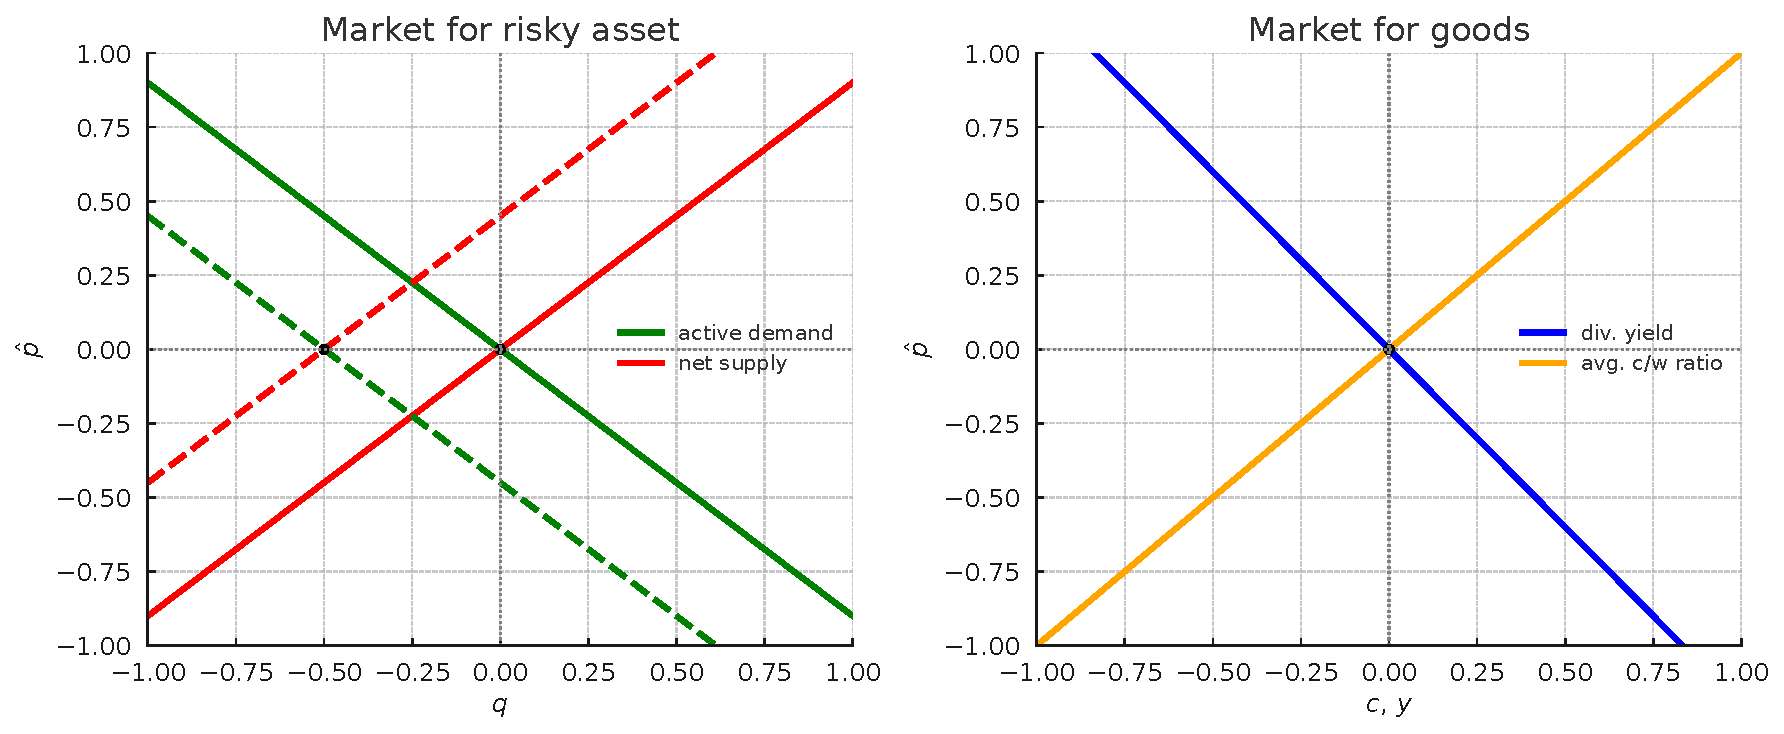
\includegraphics[width=0.95\linewidth]{figures/mkt_equilibrium.pdf}    
    \vspace{2mm}
    \caption{Equilibrium in the risky asset (left) and goods (right) markets.}
    \label{fig:mkt_equilibrium}
\end{figure}

% The left panel of Figure~\ref{fig:mkt_equilibrium} depicts the equilibrium in the market for risky asset. 
% The downward-sloping curve represents the demand from active investors. 
% The upward-sloping curve represents the net supply of risky assets, i.e., the fixed supply minus the demand from passive investors.\footnote{As passive demand is $Q_p = \overline{\alpha}_p [1- c_p(r,\mu-p-r)]\frac{P+Y}{P} Q_p$, the linearized net supply $-Q_p^\star q_p$ will be increasing in $p$ if $c_p(\cdot)$ does not react too strongly to $p$.} 

Linearizing the goods-market condition $\overline{c}(\mu-p)=1/(1+e^{p})$ around $p^\star$ yields
\begin{equation}\label{eq:goods_linear}
    \chi_p\,\hat{p}
    \;=\;
    -\,\frac{e^{p^\star}}{(1+e^{p^\star})^2}\,\hat{p},
    \qquad\text{where}\qquad
    \chi_p \equiv -\,\overline{c}'(\mu-p^\star).
\end{equation}
The right panel of Figure~\ref{fig:mkt_equilibrium} shows the goods market. We focus on the case $\chi_p>0$, so the average consumption-wealth ratio is increasing in $p$ (investors save less when expected returns are low). The right-hand side in \eqref{eq:goods_linear} is the (local) slope of the dividend-yield curve, which is downward sloping in $p$. By the recursive property, only $p$ enters the goods market clearing condition.

% \begin{figure}
%     \centering
%     % \tikzset{every picture/.style={line width=0.75pt}} %set default line width to 0.75pt        

%     \begin{tikzpicture}[x=0.75pt,y=0.75pt,yscale=-1,xscale=1]
%     %uncomment if require: \path (0,235); %set diagram left start at 0, and has height of 235

%     %Shape: Axis 2D [id:dp5132950601646007] 
%     \draw [color={rgb, 255:red, 0; green, 0; blue, 0 }  ,draw opacity=1 ][line width=1.5]  (50,200) -- (289,200)(70,39) -- (70,222) (282,195) -- (289,200) -- (282,205) (65,46) -- (70,39) -- (75,46) (101,195) -- (101,205)(132,195) -- (132,205)(163,195) -- (163,205)(194,195) -- (194,205)(225,195) -- (225,205)(256,195) -- (256,205)(65,169) -- (75,169)(65,138) -- (75,138)(65,107) -- (75,107)(65,76) -- (75,76) ;
%     \draw   ;   
%     %Straight Lines [id:da929233454246288] 
%     \draw [color={rgb, 255:red, 245; green, 166; blue, 35 }  ,draw opacity=1 ][line width=1.5]    (20,56) -- (304,218) ;
%     %Straight Lines [id:da5921961944005785] 
%     \draw [color={rgb, 255:red, 74; green, 144; blue, 226 }  ,draw opacity=1 ][line width=1.5]    (16,200) -- (276,51) ;
%     %Straight Lines [id:da2953578261472096] 
%     \draw [color={rgb, 255:red, 0; green, 0; blue, 0 }  ,draw opacity=1 ][line width=1.5]  [dash pattern={on 1.69pt off 2.76pt}]  (145,126) -- (145,200) ;
%     %Shape: Axis 2D [id:dp3699485075380834] 
%     \draw [color={rgb, 255:red, 0; green, 0; blue, 0 }  ,draw opacity=1 ][line width=1.5]  (380,200) -- (619,200)(400,39) -- (400,222) (612,195) -- (619,200) -- (612,205) (395,46) -- (400,39) -- (405,46) (431,195) -- (431,205)(462,195) -- (462,205)(493,195) -- (493,205)(524,195) -- (524,205)(555,195) -- (555,205)(586,195) -- (586,205)(395,169) -- (405,169)(395,138) -- (405,138)(395,107) -- (405,107)(395,76) -- (405,76) ;
%     \draw   ;
%     %Straight Lines [id:da7483554761171687] 
%     \draw [color={rgb, 255:red, 65; green, 117; blue, 5 }  ,draw opacity=1 ][line width=1.5]    (355,85) -- (638,222) ;
%     %Straight Lines [id:da38811786243247126] 
%     \draw [color={rgb, 255:red, 208; green, 2; blue, 27 }  ,draw opacity=1 ][line width=1.5]    (431,199) -- (460.67,36) ;
%     %Straight Lines [id:da4060861160692876] 
%     \draw [color={rgb, 255:red, 0; green, 0; blue, 0 }  ,draw opacity=1 ][line width=1.5]  [dash pattern={on 1.69pt off 2.76pt}]  (144,127) -- (504.67,127) ;
%     %Straight Lines [id:da3647922931527937] 
%     \draw [color={rgb, 255:red, 65; green, 117; blue, 5 }  ,draw opacity=1 ][line width=1.5]  [dash pattern={on 1.69pt off 2.76pt}]  (372,64.57) -- (655,201.57) ;
%     %Straight Lines [id:da21438260220121663] 
%     \draw [color={rgb, 255:red, 208; green, 2; blue, 27 }  ,draw opacity=1 ][line width=1.5]  [dash pattern={on 1.69pt off 2.76pt}]  (488,200) -- (517.67,37) ;
    
%     % Text Node
%     \draw (231,86) node  [color={rgb, 255:red, 74; green, 144; blue, 226 }  ,opacity=1 ,rotate=-329.57]  {\small $avg.\ c/w\ ratio$};
%     % Text Node
%     \draw (312,201) node  [color={rgb, 255:red, 0; green, 0; blue, 0 }  ,opacity=1 ,rotate=-358.98]  {$c,y$};
%     % Text Node
%     \draw (251,171) node  [color={rgb, 255:red, 245; green, 166; blue, 35 }  ,opacity=1 ,rotate=-28.61]  {\small $div.\ yield$};
%     % Text Node
%     \draw (54,39) node  [color={rgb, 255:red, 0; green, 0; blue, 0 }  ,opacity=1 ,rotate=-358.98]  {$p$};
%     % Text Node
%     \draw (464,63) node  [color={rgb, 255:red, 208; green, 2; blue, 27 }  ,opacity=1 ,rotate=-279.88]  {\small $net\ supply$};
%     % Text Node
%     \draw (630,201) node  [color={rgb, 255:red, 0; green, 0; blue, 0 }  ,opacity=1 ,rotate=-358.98]  {$q$};
%     % Text Node
%     \draw (552,169) node  [color={rgb, 255:red, 65; green, 117; blue, 5 }  ,opacity=1 ,rotate=-25.74]  {\small $active\ demand$};
%     % Text Node
%     \draw (384,39) node  [color={rgb, 255:red, 0; green, 0; blue, 0 }  ,opacity=1 ,rotate=-358.98]  {$p$};
%     % Text Node
%     \draw (107,4.43) node [anchor=north west][inner sep=0.75pt]   [align=left] {\textbf{Market for goods}};
%     % Text Node
%     \draw (435,3) node [anchor=north west][inner sep=0.75pt]   [align=left] {\textbf{Market for risky asset}};
% \end{tikzpicture}
%     \caption{Equilibrium in the goods and risky asset markets}
%     \label{fig:mkt_equilibrium}
% \end{figure}


\paragraph{The inelastic markets hypothesis.}
Consider a \emph{partial equilibrium} version of the model in which we hold the interest rate fixed at $r=r^\star$ and ignore goods market clearing. 
Using the linearized risky asset market condition \eqref{eq:risky_mkt_linear} with $\hat r=0$, the price of the risky asset satisfies
\begin{equation}\label{eq:mkt-elasticity-pe}
    \hat{p}
    \;=\;
    \underbrace{\frac{1}{\zeta_p}}_{\substack{\text{inverse market}\\ \text{elasticity}}}
    \times
    \underbrace{f}_{\text{flow shock}},
\end{equation}
where
\[
\zeta_p \;\equiv\; s_a\,\zeta_{a,p} + s_p\,\zeta_{p,p},
\qquad
f \;\equiv\; s_p\,f_p,
\qquad
s_j \equiv \omega_j Q_j^\star.
\]

Equation~\eqref{eq:mkt-elasticity-pe} shows that the price-dividend ratio responds to flow shocks, with price impact given by the inverse of the (aggregate) market elasticity---an average of investors’ own-price elasticities. This is the core implication of the \emph{inelastic markets hypothesis} of \citet{gabaix2020search}, who estimate large price responses to stock-market flows, suggesting relatively inelastic demand.

In the risky asset panel of Figure~\ref{fig:mkt_equilibrium}, an increase in the portfolio share of passive investors shifts the net supply curve to the left. The new equilibrium lies further up the active demand curve, implying lower expected returns and a higher price-dividend ratio. When demand is inelastic, even small inflows to stocks generate a sizable increase in $\hat{p}$.
% In the risky-asset panel of Figure~\ref{fig:mkt_equilibrium}, a reallocation by passive investors that increases their portfolio share shifts the \emph{net supply} curve to the right. The new intersection moves \emph{down} along active demand, so expected returns must rise and the price-dividend ratio falls. When investors are inelastic, even a small flow away from stocks generates a sizable decline in $\hat{p}$.

\paragraph{The crucial role of cross-elasticity.}
The partial equilibrium analysis abstracts from cross-elasticity. In general equilibrium, however, both $r$ and $p$ adjust, and the aggregate market elasticity is fundamentally different, as the next proposition shows.

\begin{prop}[Infinite market elasticity]\label{prop:inf-elasticity}
    Define the aggregate cross-elasticity $\zeta_r \;\equiv\; s_a\,\zeta_{a,r} \;+\; s_p\,\zeta_{p,r}$.
    If $\zeta_r \neq 0$, then a portfolio-flow shock has \emph{no} price impact: $\hat p=0$. The shock is absorbed by offsetting movements in the interest rate and the risk premium:
    \[
        \hat r \;=\; \frac{1}{\zeta_r}\,f, 
        \qquad 
        \hat \pi \;=\; -\,\frac{1}{\zeta_r}\,f,
    \]
    where $\hat{\pi} \equiv \pi - \pi^\star$.
\end{prop}
\begin{proof}
    From Equation~\eqref{eq:goods_linear}, we obtain $\hat{p} = 0$. 
    If $\zeta_r \neq 0$, then $\hat{r} = \frac{1}{\zeta_r} f$ from Equation~\eqref{eq:risky_mkt_linear}.    
    Since $\hat \pi = -\hat p - \hat r$ with $\hat p=0$, it follows that $\hat \pi = - f/\zeta_r$.
\end{proof}

With any nonzero cross-elasticity $\zeta_r \neq 0$, the aggregate market becomes infinitely elastic, regardless of how inelastic individual demands may be. Even if $\zeta_{j,p}^q \approx 0$ for all $j$, a small but positive $\zeta_r$ is sufficient to make aggregate elasticity unbounded.
%With any nonzero cross-elasticity, $\zeta_r\neq 0$, the market is \emph{infinitely elastic}, regardless of how inelastic individual demands (own-price elasticities) may be. Even if $\zeta_{j,p}^q \approx 0$ for all $j$, a small but positive $\zeta_r$ suffices to make the aggregate elasticity infinite.

The disconnect between individual and aggregate elasticities arises from a general equilibrium effect. In the goods market (right panel of Figure~\ref{fig:mkt_equilibrium}), the price-dividend ratio is determined by consumption behavior. This mechanism is well known in the macro-finance literature, most clearly in models with unit EIS, where $p$ is tied directly to the discount rate. Our framework generalizes this logic. To restore equilibrium in the risky asset market (left panel), the interest rate adjusts so that active demand equals net supply at the \textit{original price}. Graphically, this appears as the dashed active-demand curve shifting to intersect the new net-supply curve at the initial price.
% This disconnect between individual and aggregate elasticities is a result of a general equilibrium effect. In the goods market (right panel of Figure~\ref{fig:mkt_equilibrium}), the price-dividend ratio is pinned down by consumption behavior. 
% This is a pervasive feature in the macro-finance literature, which is most clearly seen in unit EIS models, where $p$ is tied to the discount rate. Our formulation simply extends this logic more broadly. 
% To restore equilibrium in the risky-asset market (left panel), the interest rate adjusts so that active demand meets net supply at the \emph{original} price. In the diagram, this appears as the dashed active-demand schedule shifting until it intersects the new net-supply curve at the initial price.

Consider a positive flow shock to the risky asset (e.g., funds shift toward stocks, so $f>0$). Lower bond demand increases $r$, while increased demand for the risky asset reduces the risk premium. In equilibrium these effects offset exactly, leaving the price-dividend ratio unchanged. If the rise in $r$ were smaller than the fall in the risk premium, there would be excess demand for goods (equivalently, excess bond supply). Simultaneous clearing of risky and risk-free asset markets therefore requires infinite aggregate elasticity in this model.
%Intuitively, consider a negative flow shock to the risky asset (e.g., funds move toward bonds, so $f<0$). The increased bond demand pushes $r$ down, while the reduced demand (or higher net supply) for the risky asset raises the risk premium. In equilibrium these two forces offset \emph{exactly}, leaving the price–dividend ratio unchanged. If the decline in $r$ were too small relative to the increase in the risk premium, there would be excess demand for goods (equivalently, excess bond supply). Simultaneous clearing in the risky and riskless asset markets thus requires infinite aggregate elasticity in this model.

\paragraph{The need for a micro-founded demand system.}
The analysis underscores the central role of cross-price elasticity. The aggregate market can be infinitely elastic—even if individual investors are inelastic—so long as the average consumption-wealth ratio is unaffected by the flow shock $f$. When the flow shock shifts both the net-supply curve and the average consumption-wealth ratio, prices adjust and aggregate elasticity becomes finite.\footnote{An analogous argument applies to uncertainty. With unit EIS, the consumption–wealth ratio is fixed, so higher uncertainty leaves prices unchanged. For uncertainty to reduce prices, EIS must exceed one so that higher uncertainty lowers the consumption–wealth ratio \citep[see][]{bansal2004risks}.}  

Understanding aggregate elasticity therefore requires a framework that links portfolio reallocation shocks to both risky asset demand and bond demand (i.e., savings behavior). To this end, we develop a dynamic heterogeneous-agent asset pricing model and introduce a new methodology for deriving investor demand within this setting.

% The analysis above highlights the central role of cross-price elasticity. It shows that the aggregate market can be infinitely elastic—even when individual investors are inelastic—provided the average consumption-wealth ratio is unchanged by the portfolio flow shock $f$. If the flow shock shifts \emph{both} the net-supply schedule and the average consumption-wealth ratio, prices respond and aggregate elasticity is finite.\footnote{A similar logic applies to changes in uncertainty. When the EIS equals one and the consumption–wealth ratio is fixed, higher uncertainty leaves the price unchanged. For uncertainty to lower the price, a high EIS is required so that higher uncertainty reduces the consumption–wealth ratio (see, e.g., \citealt{bansal2004risks}).}

% Understanding the determinants of aggregate elasticity therefore requires a theory that links portfolio reallocation shocks to \emph{both} risky asset demand and bond demand (i.e., savings behavior). To this end, we develop a dynamic heterogeneous-agent asset pricing model and introduce a new methodology to derive investor demand within this framework.
